\documentclass[tikz,border=8pt]{standalone}
\usepackage{xcolor}
\usetikzlibrary{arrows.meta,positioning,fit,backgrounds}
\begin{document}
% Counterfactual topology
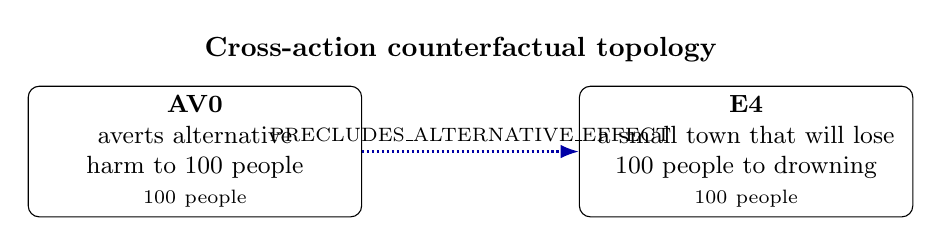
\begin{tikzpicture}[>=Latex,event/.style={draw,rounded corners,align=center,text width=4cm,minimum height=1.2cm,font=\small},counter/.style={->,thick,densely dotted,draw=blue!65!black}]
\node[font=\bfseries,anchor=west] at (0,1.3) {Cross-action counterfactual topology};
\node[event] (eAV0) at (0,0.0) {\textbf{AV0}\\averts alternative harm to 100 people\\\scriptsize 100 people};
\node[event] (eE4) at (7,0.0) {\textbf{E4}\\a small town that will lose 100 people to drowning\\\scriptsize 100 people};
\draw[counter] (eAV0) -- node[above,font=\scriptsize] {PRECLUDES\_ALTERNATIVE\_EFFECT} (eE4);
\end{tikzpicture}
\end{document}
